
\documentclass[man]{apa6}
\usepackage{lmodern}
\usepackage{amssymb,amsmath}
\usepackage{ifxetex,ifluatex}
\ifnum 0\ifxetex 1\fi\ifluatex 1\fi=0 % if pdftex
  \usepackage[T1]{fontenc}
  \usepackage[utf8]{inputenc}
\else % if luatex or xelatex
  \ifxetex
    \usepackage{mathspec}
  \else
    \usepackage{fontspec}
  \fi
  \defaultfontfeatures{Ligatures=TeX,Scale=MatchLowercase}
\fi
% use upquote if available, for straight quotes in verbatim environments
\IfFileExists{upquote.sty}{\usepackage{upquote}}{}
% use microtype if available
\IfFileExists{microtype.sty}{%
\usepackage{microtype}
\UseMicrotypeSet[protrusion]{basicmath} % disable protrusion for tt fonts
}{}
\usepackage{hyperref}
\hypersetup{unicode=true,
            pdftitle={Syntactic or morphological bootstrapping?: A cross-linguistic study},
            pdfauthor={Ebru Ger, Aylin C. Küntay, Tilbe Göksun, Sabine Stoll, \& Moritz M. Daum},
            pdfkeywords={keywords},
            pdfborder={0 0 0},
            breaklinks=true}
\urlstyle{same}  % don't use monospace font for urls
\usepackage{graphicx,grffile}
\makeatletter
\def\maxwidth{\ifdim\Gin@nat@width>\linewidth\linewidth\else\Gin@nat@width\fi}
\def\maxheight{\ifdim\Gin@nat@height>\textheight\textheight\else\Gin@nat@height\fi}
\makeatother
% Scale images if necessary, so that they will not overflow the page
% margins by default, and it is still possible to overwrite the defaults
% using explicit options in \includegraphics[width, height, ...]{}
\setkeys{Gin}{width=\maxwidth,height=\maxheight,keepaspectratio}
\IfFileExists{parskip.sty}{%
\usepackage{parskip}
}{% else
\setlength{\parindent}{0pt}
\setlength{\parskip}{6pt plus 2pt minus 1pt}
}
\setlength{\emergencystretch}{3em}  % prevent overfull lines
\providecommand{\tightlist}{%
  \setlength{\itemsep}{0pt}\setlength{\parskip}{0pt}}
\setcounter{secnumdepth}{0}
% Redefines (sub)paragraphs to behave more like sections
\ifx\paragraph\undefined\else
\let\oldparagraph\paragraph
\renewcommand{\paragraph}[1]{\oldparagraph{#1}\mbox{}}
\fi
\ifx\subparagraph\undefined\else
\let\oldsubparagraph\subparagraph
\renewcommand{\subparagraph}[1]{\oldsubparagraph{#1}\mbox{}}
\fi

%%% Use protect on footnotes to avoid problems with footnotes in titles
\let\rmarkdownfootnote\footnote%
\def\footnote{\protect\rmarkdownfootnote}


  \title{Syntactic or morphological bootstrapping?: A cross-linguistic study}
    \author{Ebru Ger\textsuperscript{1}, Aylin C. Küntay\textsuperscript{2}, Tilbe
Göksun\textsuperscript{2}, Sabine Stoll\textsuperscript{3}, \& Moritz M.
Daum\textsuperscript{1,4}}
    \date{}
  
\shorttitle{Causal sentence-event mapping}
\affiliation{
\vspace{0.5cm}
\textsuperscript{1} Department of Psychology, University of Zurich\\\textsuperscript{2} Department of Psychology, Koç University\\\textsuperscript{3} Institute of Comparative Linguistics, University of Zurich\\\textsuperscript{4} Neuroscience Center Zurich, University of Zurich and ETH Zurich}
\keywords{keywords\newline\indent Word count: X}
\usepackage{upgreek}
\captionsetup{font=singlespacing,justification=justified}

\usepackage{longtable}
\usepackage{lscape}
\usepackage{multirow}
\usepackage{tabularx}
\usepackage[flushleft]{threeparttable}
\usepackage{threeparttablex}

\newenvironment{lltable}{\begin{landscape}\begin{center}\begin{ThreePartTable}}{\end{ThreePartTable}\end{center}\end{landscape}}

\makeatletter
\newcommand\LastLTentrywidth{1em}
\newlength\longtablewidth
\setlength{\longtablewidth}{1in}
\newcommand{\getlongtablewidth}{\begingroup \ifcsname LT@\roman{LT@tables}\endcsname \global\longtablewidth=0pt \renewcommand{\LT@entry}[2]{\global\advance\longtablewidth by ##2\relax\gdef\LastLTentrywidth{##2}}\@nameuse{LT@\roman{LT@tables}} \fi \endgroup}


\DeclareDelayedFloatFlavor{ThreePartTable}{table}
\DeclareDelayedFloatFlavor{lltable}{table}
\DeclareDelayedFloatFlavor*{longtable}{table}
\makeatletter
\renewcommand{\efloat@iwrite}[1]{\immediate\expandafter\protected@write\csname efloat@post#1\endcsname{}}
\makeatother
\usepackage{lineno}
\usepackage{csquotes}
\usepackage{apacite}

\linenumbers
\raggedbottom

\authornote{We thank the participants, their parents and the
kindergartens for their participation. We also thank Larissa Stuber,
Sura Ertaş, Sena Gezici, Merve Duran, and Raphaela Schnider for their
thoughtful contribution and help in data collection and coding. This
work was funded by the Swiss National Foundation (XXX).

Correspondence concerning this article should be addressed to Ebru Ger,
Department of Psychology, Binzmuehlestrasse 14, Box 21, 8050 Zurich,
Switzerland. E-mail:
\href{mailto:e.ger@psychologie.uzh.ch}{\nolinkurl{e.ger@psychologie.uzh.ch}}}

\abstract{
To be written..

One or two sentences providing a \textbf{basic introduction} to the
field, comprehensible to a scientist in any discipline.

Two to three sentences of \textbf{more detailed background},
comprehensible to scientists in related disciplines.

One sentence clearly stating the \textbf{general problem} being
addressed by this particular study.

One sentence summarizing the main result (with the words ``\textbf{here
we show}'' or their equivalent).

Two or three sentences explaining what the \textbf{main result} reveals
in direct comparison to what was thought to be the case previously, or
how the main result adds to previous knowledge.

One or two sentences to put the results into a more \textbf{general
context}.

Two or three sentences to provide a \textbf{broader perspective},
readily comprehensible to a scientist in any discipline.


}

\begin{document}
\maketitle

deneme

How do children learn causal verbs? Syntactic bootstrapping hypothesis
has been suggested and widely investigated as one mechanism for how
children acquire new causal verbs. This hypothesis proposes that the
syntactic structure of a sentence serves as a cue to the meaning of words in the
sentence \cite{gleitman1990structural} (Gleitman, 1990; Landau, Gleitman, \& Landau,
2009). In line with this hypothesis, transitive sentence frame (i.e.~containing two
noun phrases) has been documented as a linguistic cue to causality that
adults and children make use of to map form to meaning (Fisher, 1996,
2002; Fisher, Hall, Rakowitz, \& Gleitman, 1994; Kline, Snedeker, \&
Schulz, 2017; Lidz, Gleitman, \& Gleitman, 2003; Naigles, 1990; Naigles \& Kako,
1993). For example, Kline et al. (2017) found that when
children were asked a question with a nonsense verb in a transitive
frame (e.g.~where did the girl \emph{gorp} the tall thing?) they chose a
causal scene where a puppet touches an object and immediately makes it
work rather than a non-causal scene where the puppet stops short of
touching the object, which works after a slight delay, evincing the use
of the transitive syntactic frame to derive causal meanings. However,
languages differ in terms of the types of existing cues to causality as
well as the availability and reliability of these cues to hint
causality. For example, some languages such as Kannada or Turkish attach
a distinct causative morpheme to verbs to express causality, alongside
the transitive syntactic structure that cues causality. These verbal
causative markers are fully reliable to denote causality unlike a
transitive sentence frame which can also denote non-causal events such
as in the sentence \enquote{I see her} (Göksun, Küntay, \& Naigles,
2008; Lidz et al., 2003). Furthermore, some languages such as Mandarin
or Turkish allow extensive noun ellipsis, resulting in the occasional
unavailability of the syntactic cue in causal sentences (Göksun et al.,
2008; Lee \& Naigles, 2005, 2008). The type of existing causality cues
in a given language as well as the availability and reliability of these
cues within each language might influence the extent to which children
make use of each potential cue to learn causal verbs. Given these
differences across languages that might influence the strength of
possible bootstrapping mechanisms on the learning of causal verbs, it is
necessary to revisit the syntactic bootstrapping hypothesis by taking a
cross-linguistic approach.

In the current study we examine two typologically distinct languages
with different cue characteristics for causality, namely Turkish and
Swiss-German. We test the ability of Turkish-speaking children and Swiss-German-speaking children to use the causality cues in their
respective languages to map onto causal events (For brevity hereafter
referred to as \enquote{Turkish} and \enquote{Swiss}). Specifically,
we investigate whether syntactic frame is a sufficient universal cue
children benefit from to learn causal verbs in the early phase of their
language acquisition irrespective of its availability in a given language,
and whether language-specific cues with absolute reliability, such as the
verbal causative marker, provide an equally sufficient exclusive benefit
or a supplementary benefit in learning causal verbs. In what follows, we
explain the characteristics of the causality cues in Turkish and Swiss-German.

In Turkish, causality is mainly expressed with verbal morphological
constructions. A causative morpheme can be productively affixed to any
verb stem resulting in a highly regular causativization process
(Shibatani \& Pardeshi, 2002). For example, an intransitive verb such as
in (1) can be causativized with the causative marker \enquote{-dir} as
in (2).\footnote{The vowels in suffixes are subject to change based on
  the verb root, due to vowel harmony rules in Turkish (Kabak, 2011).}
The causative morphemes are absolutely reliable to express causality when they are present. In addition, the presence of two noun phrases in a sentence as in (2) serves as a syntactic cue to causality (Göksun et al., 2008). Consequently, sentences as (2) provide a combination of syntactic and
verbal morphological cues to causality.

\begin{enumerate}
\def\labelenumi{(\arabic{enumi})}
\tightlist
\item
  \emph{Ali gül-dü.}\\
  Ali laugh-PAST.3SG\\
  \enquote{Ali laughed.}
\end{enumerate}

\newpage

\begin{enumerate}
\def\labelenumi{(\arabic{enumi})}
\setcounter{enumi}{1}
\tightlist
\item
  \emph{Arda Ali-yi gül-dür-dü.}\\
  Arda Ali-ACC laugh-CAUS-PAST.3SG\\
  \enquote{Arda made Ali laugh.}
\end{enumerate}

However, Turkish also contains lexical causatives, which are causal
verbs that inherently express a causal meaning without any causal marker
attached, as in (3). Such sentences contain the syntactic cue but
not the verbal morphological cue to causality.

\begin{enumerate}
\def\labelenumi{(\arabic{enumi})}
\setcounter{enumi}{2}
\tightlist
\item
  \emph{Ali kalem-i kır-dı.}\\
  Ali pencil-ACC break-PAST.3SG\\
  \enquote{Ali broke the pencil.}
\end{enumerate}

Furthermore, Turkish allows pervasive noun ellipsis such that either or
both of the noun phrases in a causal sentence can be omitted. Hence a
sentence involving a causatively marked verb with a single noun phrase
(e.g.~the subject), such as in (4), would contain a verbal morphological
cue but lack a syntactic cue to causality.

\begin{enumerate}
\def\labelenumi{(\arabic{enumi})}
\setcounter{enumi}{3}
\tightlist
\item
  \emph{Arda gül-dür-dü.}\\
  Arda laugh-CAUS-PAST.3SG\\
  \enquote{Arda made {[}0{]} laugh.}
\end{enumerate}

Moreover, Turkish employs nominal case marking that serves as yet
another cue to causality (Göksun et al., 2008), with the accusative
markers denoting the patient (i.e.undergoer) of a causal action, as in
(2) and (3). Nonetheless, it is possible to form causal sentences
without the accusative marker yet with two noun phrases, when the direct
object has an indefinite or a non-specific status (Erguvanli \& Taylan,
1984; Ketrez, 2004), such as \enquote{\emph{bir elma} (an apple)} in
(5). In this study, we aimed to examine the role of syntactic and verbal
morphological causality cues on causal form to meaning mapping,
independent of the effect of nominal case markers. Therefore, we used
indefinite direct objects in our stimuli.

\begin{enumerate}
\def\labelenumi{(\arabic{enumi})}
\setcounter{enumi}{4}
\tightlist
\item
  \emph{Ali bir elma ye-di.}\\
  Ali an apple eat-PAST.3SG\\
  \enquote{Ali ate an apple.}
\end{enumerate}

Swiss-German expresses causality mainly with lexical causatives and does
not employ verbal morphological constructions of causality unlike
Turkish. In addition, it does not employ a distinctive nominal case
marking as in standard German. Together, it serves as an optimal
comparison base by enabling us to form causal sentences containing only
a syntactic cue to causality, as in (6). Furthermore, the syntactic
frame cue to causality is always present since Swiss-German does not allow noun
ellipsis as in Turkish. Thus, we can examine the influence of the
availability of syntactic cues by comparing Swiss-German, in which it is
always available, and Turkish in which it is not always available.

\begin{enumerate}
\def\labelenumi{(\arabic{enumi})}
\setcounter{enumi}{5}
\tightlist
\item
  \emph{De Pascal het de Bleistift g-schlisse.}\\
  Pascal has the pencil break-PAST.PERF\\
  \enquote{Pascal broke the pencil.}
\end{enumerate}

In the following two sections we review the literature focusing on the
effects of verbal morphology and noun ellipsis on deriving causal
meanings.

\subsection{Verbal Morphology}\label{verbal-morphology}

A few studies investigated how children enacted sentences consisting of
different, and sometimes conflicting, cues to causality. Lidz et al.
(2003) approached the syntactic bootstrapping hypothesis from a
comparative stance. They pitted the universalist view of verb
acquisition against the emergenist view under this hypothesis. The
universalist view argues that syntax-semantics interface is inherently
present in every language system and serves as the primary framework for
children in verb learning. The emergenist view argues that the
syntax-semantics interface is learned through the input and that
language-specific properties of a language serve as the primary guide
towards verb learning. They measured the causative act-outs upon hearing
sentences consisting of conflicting cues to causality in speakers of
Kannada, a Dravidian language (spoken mainly in southern India and parts
of eastern and central India) where the most reliable cue to causality
is a causative morpheme affixed to verbs. For example, they asked
children to enact sentences such as \enquote{The lion goes the zebra}.
They hypothesized that the emergenist account would predict the learners
of this language to rely more on this more reliable language-specific
cue whereas the universalist account would predict the syntactic frame
(i.e., the noun phrases in the sentence denoting the agent and the
patient) to prevail over verbal morphology. They found that 3-year-old
Kannada speakers relied on the syntactic frame rather than the verbal
morphology in providing causative act-outs when these cues competed,
supporting the universalist account. In a similar vein, Göksun et al.
(2008) examined the causative act-outs of 2- to 5-year-old children
speaking Turkish, which is another language where the most reliable cue
to causality is a causative morpheme. They also found that children
relied more on the syntactic frame than the causative morpheme. These
results suggest a universal superiority of the syntactic frame; however,
certain language-specific characteristics, such as noun ellipsis, can
challenge these results. Next, we turn to the topic of noun ellipsis in
relation to syntactic bootstrapping.

\subsection{Noun Ellipsis}\label{noun-ellipsis}

The majority of the empirical findings on the syntactic bootstrapping
account come from languages that are fixed in terms of the number and
order of the noun phrases in a causative sentence, such as English and
French (Naigles \& Lehrer, 2002). However, other languages such as
Mandarin, Japanese, or Turkish allow pervasive noun ellipsis. In such
languages, the syntactic frame is not always available to map onto
causal meanings as it is perfectly plausible to form causal sentences
with no arguments or a single argument, where the information about the
arguments can be drawn from the surrounding non-linguistic or discourse
context. In fact, in child-directed speech, utterances lacking one or
two arguments were observed frequently in Turkish (Küntay \& Slobin,
1996) and in Japanese (Rispoli, 1995). This lack was suggested to pose a
potential difficulty for the functioning of the syntactic bootstrapping
mechanism (Bowerman \& Brown, 2008). Nonetheless, for example in Turkish
child-directed speech, the number of nominals were found to be
moderately effective in distinguishing between transitive and
intransitive verbs by a machine-learning algorithm (Ural, Yuret, Ketrez,
Koçbaş, \& Küntay, 2009). Further, in similar act-out studies, both
Mandarin-speaking children (Lee \& Naigles, 2008) and Turkish-speaking
children (Göksun et al., 2008) were found to causatively enact
intransitive verbs more often in two noun phrase sentences compared to
one noun phrase sentences; and non-causatively enact transitive verbs
more often in one noun phrase sentences compared to two noun phrase
sentences. Hence, children were able to make use of the two noun phrases
to map the verbs onto causal meanings although their native language
input does not provide a consistency for the number of noun phrases with
which causality is expressed, due to noun ellipsis. These findings
support the view that syntactic bootstrapping is a sufficiently strong,
universal, and perhaps innate cue for deriving causal meanings (Chomsky,
1964; Pinker, 2009). Nonetheless, another study comparing children
speaking English, Mandarin and Turkish found that the latter two were
less frame-compliant, and displayed verb-compliance earlier than English
speakers, perhaps due to the noun ellipsis in these languages (Naigles,
Küntay, Göksun, \& others, 2006). Therefore, the specific input
characteristics of languages might still matter, at least for the
extent to which syntactic cues are utilized to map onto causal meanings.

\subsection{Current Study}\label{current-study}

An important limitation of the reviewed studies focusing on the
syntactic frame and the verbal morphology with regard to causativity is
that they employed familiar transitive and intransitive verbs that were
either compliant or incompliant with the syntactic frame. Therefore, the
effect of syntax or verbal morphology on causative act-outs was not
independent of the verb semantics. They were able to observe if children
acted out in a verb-compliant manner (e.g.~moving only the zebra upon
hearing \enquote{The zebra goes the lion}) or frame-compliant manner
(e.g.~moving only the zebra upon hearing \enquote{The zebra brings})
when the verb and the frame information conflicted but not the extent to
which children can make use of different structural cues to learn verb
meanings when the cues do not conflict. To be able to examine the
bootstrapping of syntax versus verbal morphology in learning of causal
verbs, the use of pseudo-verbs would be useful to disentangle the effect of
structure from semantics. Additionally, participants' causative or
non-causative choices in act-outs upon hearing conflicting cues hinder a
clear comparison between the effect of each cue. For example, how well a
child knows the meaning of a verb or the frequency of a verb in the language
might affect the extent to which the child is willing to act out in a
verb-compliant manner by ignoring the syntactic structure which conflicts
with the verb valence. Therefore, cross-linguistic comparisons employing
languages that have different availability and reliability of cues instead
of using cues in conflicting ways within a language and using pseudo-verbs
instead of familiar verbs is a promising approach to test the influence
of different grammatical cues on mapping form to meaning. Consequently
we address the following three questions in our study:

\begin{enumerate}
\def\labelenumi{\arabic{enumi}.}
\item
  Do Turkish children and Swiss children differ in their performance of
  mapping sentences to causal scenes if Turkish sentences contain both
  syntactic as well as verbal morphological causality cues and
  Swiss-German sentences contain only syntactic causality cues?
\item
  Do Turkish children and Swiss children differ in their performance of
  mapping sentences to causal scenes if Turkish sentences and
  Swiss-German sentences both contain only syntactic causality cues?
\item
  Do Turkish children and Swiss children differ in their performance of
  mapping sentences to causal scenes if Turkish sentences contain only
  verbal morphological causality cues and Swiss-German sentences
  contain only syntactic causality cues?
\end{enumerate}

We form our hypotheses on these questions from a comparative stance as
in Lidz et al. (2003). However, a limitation of this study is that when
pitting universalist and emergenist accounts against each other, they
took only the reliability of cues into account to derive their
hypotheses on the emergenist account. However, the availability and
reliability of each cue in a given language can have a combined effect
on how well that cue is utilized to bootstrap meaning. Hence, we exploit
the Competition Model by Bates and MacWhinney (1989) that takes
into account the availability and reliability of cues in a language to
form our hypotheses under the emergenist approach. This model proposes
that the validity of a cue determines whether that cue is preferred as a
guide to interpret sentence meanings amongst other cues. The cue
validity is composed of cue availability and cue reliability and is
operationalized as the multiplication of the values of the latter two.
The cue availability is how often a cue is present in a sentence to
interpret the meaning it cues. For example, in English nominative case
marking is available only with pronouns to cue actor role in sentences
with a transitive frame. The cue reliability is how often a cue
correctly identifies the meaning it cues. For example, in English word
order is a highly reliable cue for determining agent-patient roles in a
causative sentence (e.g. \enquote{She kissed him} would be typical
sentence whereas we encounter sentences like \enquote{Him kissed she}
only in poetry).

In forming our hypotheses under the universalist approach, we take on
the premise of the superiority of syntax in expecting a better
performance in sentences with an intact transitive syntactic frame,
regardless of its availability in a given language to express causality.
In forming our hypotheses under the emergenist view, we first evaluate
the validity components of the examined cues in both Turkish and
Swiss-German. To contemplate on the validity of syntax as a cue to
causality in Turkish and Swiss-German, we focus on the availability and
reliability of this cue in each language. In Swiss-German, transitive
sentence frame is always present as a cue to causality. However, in
Turkish, syntax is not always available as a cue to causality due to
noun ellipsis. For both languages, although syntax is a highly reliable
cue to causality as most of the transitive sentences express causality,
it is not always reliable as there are non-causative transitive verbs
such as \enquote{see (\enquote{-gör} in Turkish, \enquote{gseh} in
Swiss-German)}. The validity of the causative marker as a cue to
causality in Turkish can be drawn from the availability and reliability
of this cue. Since there are lexical causatives such as \enquote{-kır
(break)} or \enquote{-it (push)} which are verbs that readily denote a
causal event in its root form, causative marker is not always available
in causal sentences. However, the causative marker is a 100\% reliable
cue because it expresses a causal meaning whenever it is present.

For the first question, the universalist account predicts that the
Turkish children would not perform differently in mapping the sentences
to corresponding events than Swiss children, given that both groups have
the syntax cue. The emergenist account predicts that the Turkish
children would perform worse than Swiss children. Because, although in
Turkish the combination of transitive frame and verbal morphological
cues expresses causality with a 100\% reliability, the availability of
this combination for causal sentences is expected to be low given the
lexical causatives and noun ellipsis. Whereas in Swiss-German, syntax is
a fully available and highly (albeit not fully) reliable cue for
causality.

For the second question, the universalist account predicts that the
Turkish children would not perform differently than Swiss children,
given that both groups have the syntax cue. The emergenist account would
predict that the Turkish children would perform worse than Swiss
children. Because, albeit not fully reliable, syntax is always available
as a cue to causality in Swiss-German whereas in Turkish it is not a
fully reliable cue as well as not always available due to noun ellipsis.

For the third question, the universalist account predicts that the
Turkish children would perform worse than Swiss children, given that
Turkish children lack the syntax cue. The emergenist account would
predict that the Turkish children would not perform differently than
Swiss children. Because, although the verbal morphology cue in Turkish
is fully reliable it is not fully available; and although the syntax cue
in Swiss-German is fully available it is not fully reliable. Therefore,
the validity of the verbal morphology cue in Turkish and the syntax cue
in Swiss-German would be at comparable levels.

\section{Methods}\label{methods}

As stated in our pre-registration, our target sample was determined upon
power analyses for a priori sample size requirements performed on the
G*power software. The relevant literature was reviewed for effect sizes.
When they were not reported, the effect size conversion spreadsheet
created by Daniel Lakens (\url{http://osf.io/ixgcd/}) was used to
calculate them from reported statistics. All the relevant studies
reviewed had medium to large effect sizes with r values ranging from
0.32 to 0.60. We set our smallest effect size of interest as r = 0.32
(transformed to Cohen's d = 0.68) and our power to 0.90 for the power
analysis of a planned one-way ANCOVA with the language + condition
groups as the independent variable with 4 categories and, age and
receptive vocabulary as the covariates. We planned three one-tailed
analyses for the planned comparisons (to test our 3 hypotheses listed at
the end of the introduction part), therefore we set our type 1 error
rate to 0.016, applying a Bonferroni correction for the alpha level of
0.05 for three pairwise comparisons. The study we adopted our design
from, Kline et al. (2017), had a non-normal distribution of the
dependent variable with 3 to 4-year-old English speakers, therefore we
similarly expected a non-normal distribution and foresaw the use of
Wilcoxon-Mann-Whitney tests for our planned comparisons. Given these
parameters, the sample size calculated per group was 45.

We had a pretest pass criteria, that is, children were included in the
final analyses for the mapping performance only if they correctly
answered at least 3 out of the 4 pretest questions that were aimed at
determining if children understood the causality/non-causality in the
scenes. Children who failed the pretest were replaced. However, the
number of children that failed to pass the pretest were far more than
expected based on the original study we adapted. Therefore, we decided
to also analyze the performance of the children who failed the pretest
in comparison to those who passed, in order to see if understanding the
causality in scenes was an essential part of the bootstrapping effect of
linguistic causal cues in mapping novel causal verbs into their semantic
correspondences.

\subsection{Participants}\label{participants}

Based on Kline et al. (2017), we tested 3- to 4-year-old (36 to 59
months) typically developing monolingual Turkish and Swiss children. Our
criteria for typical development was the absence of any parent-reported
developmental problems that would pose a potential decrease in
children's performance in our tasks, such as language or hearing related
problems. Swiss participants were recruited via the participant database
of the University of Zurich, Chair of Developmental Psychology: Infancy
and Childhood, and the children were presented with a small gift and a
symbolic certificate for their participation. Turkish participants were
recruited from kindergartens in Istanbul, Turkey and were presented with
a small gift for their participation. A demographic form was obtained
from children's parents asking whether children were exposed to an
additional language than the target language, and if so, the percentage
of the exposure. Children were not tested if the exposure to (an)
additional language(s) exceeded 15\%.

We replaced children who failed to pass the pretest until we obtained
this target sample size. In total, we tested 189 Turkish and 72 Swiss
children. We excluded 18 Turkish children (8 developmental problems, 5
technical error, 1 fuss, 4 younger than the target age range) and 6
Swiss children (fussed). Out of the remaining 171 Turkish children 36
failed the pretest (16 verbal morphological, 10 syntactic, 10 syntactic
plus verbal morphological). Out of the remaining 66 Swiss children 21
failed the pretest.

In the analyses where we examined the effect of passing the pretest on
children's performance, we included 171 Turkish children (79 female,
\emph{M}\textsubscript{age} = 46.73 months, \emph{SD} = 5.33) and 66
Swiss children (34 female, \emph{M}\textsubscript{age} = 49.20 months,
\emph{SD} = 5.67). In the final analyses we included 135 Turkish
children (65 female, \emph{M}\textsubscript{age} = 47.20 months,
\emph{SD} = 5.27), and 45 Swiss children (21 female,
\emph{M}\textsubscript{age} = 50.24 months, \emph{SD} = 5.27).

\subsection{Material}\label{material}

For the training phase of the experiment, we used a female puppet and a
remote-controlled toy cement truck whose container could rotate, which
was attached on a cardboard box with an opening on the back. The remote
control and its cable was hidden inside the box through this opening to
allow the experimenter to secretly operate the toy. A 17-inch Lenovo
touchscreen laptop was used for the main experiment and the receptive
vocabulary test. Both tests were run in PsychoPy (Peirce \& MacAskill,
2018). For the pretest and test phase of the experiment we used the
stimuli video from Kline et al. (2017) and added voiceover of prompts in
our tested languages. The pretest and test videos consisted of the
causal and non-causal version of an event, where the same puppet as in
the training phase touched an unfamiliar toy that could move or light up
or make a sound, and immediately made it activate (causal) or the puppet
stopped short of touching the toy and the toy activated after a 1 second
delay (non-causal). There was one pair of events in the pretest phase
and four pairs of events in the test phase. After the pretest video pair
children heard a positive and a negative version of two questions; and
after the test video pairs they heard a positive and a negative version
of a prompt. The pairs of each event were presented one by one on the
left and right hand side of the computer screen. The presentation order
of the events and the sides were randomized. See the materials section
under each language and condition folder to view the corresponding
videos and prompts with the following link: \url{https://osf.io/aytnx/}
(\enquote{event1c} and \enquote{event1n} respectively depicts the
causal and non-causal pretest videos; \enquote{event3c} trough
\enquote{event4c} depict the causal test videos, \enquote{event3n}
through \enquote{event6n} depict the non-causal test videos;
\enquote{preq1pos} and \enquote{preq1neg} respectively depict the causal
and non-causal version of pretest question 1, \enquote{preq2pos} and
\enquote{preq2neg} respectively depict the causal and non-causal version
of pretest question 2; \enquote{positive3} through \enquote{positive6}
depict the causal test prompts, \enquote{negative3} through
\enquote{negative6} depict the non-causal test prompts).

\subsection{Procedure}\label{procedure}

Swiss children were tested in the lab at the University of Zurich in
Switzerland; Turkish children were tested in a quiet room in
kindergartens around Istanbul, Turkey. On the Swiss site, children and
parents were first welcomed to a play room in the lab where the child
and the experimenter warmed up by playing games for several minutes.
Then they were escorted to a testing room. On the Turkish site, the
experimenter was introduced to the children in a classroom in the
kindergarten and participating children were taken to a quiet room
individually. The experimenter warmed up with the child by conversing
for a few minutes before starting testing. On both sites, the child sat
in front of a table facing the experimenter; and only on the Swiss site
the parent sat behind the child. Children were videotaped by two cameras
at the front and the back of the child.

The testing consisted of a training phase, a pretest phase and a test
phase. The training phase aimed at teaching the child that a toy might
sometimes move on its own but sometimes can be caused to move by
someone. Firstly, the experimenter told the child that
\enquote{sometimes the toy moves when the girl and the toy touch} and
she brought the puppet towards the toy, made its hand touch the surface
of the box right next to where the toy stood and immediately activated
the toy and said \enquote{like this, she makes the toy move} (repeated
twice). Then she offered the child to try by moving the toy closer to
the child and once the child touched the toy she activated it. If the
child kept on touching after a few seconds, the experimenter asked the
child to remove his hand. If the child still did not remove his hand,
the experimenter gently removed the toy from him. Afterwards, the
experimenter said that \enquote{sometimes the toy moves on its own while
the girl just watches}, tilted the puppet towards the toy, activated the
toy after a brief pause, and said \enquote{like this, because it has a
battery inside} (repeated twice).

Then the pretest phase started. After watching each video, the
experimenter pointed to the video and asked the child: \enquote{In this
video, did the girl and the green toy touch or not touch?} If the child
answered correctly she moved to the second question and asked:
\enquote{In this video did the girl make the green toy squeak or did the
toy squeak on its own?} If the child answered correctly she moved on to
play the other video and asked the same questions. If the child
responded incorrectly or did not respond to either of the questions she
gave feedback by saying the correct answer as \enquote{Hmm, I think in
this video the girl and the green toy touched/did not touch} and
\enquote{Hmm, I think in this video the girl made the green toy
squeak/the green toy squeaked on its own}. Then she repeated the video
and asked the unanswered/incorrectly answered question(s) again. The
same video was repeated only once more if the child did not answer or
incorrectly answered the question. Then the experimenter told the child
that they would practice pointing. The child heard the positive and
negative versions of two questions. One question asked where the puppet
and the toy (do not) touch (\enquote{preq1pos},\enquote{preq1neg}) and the other question asked where the girl (did not make) made the toy squeak (\enquote{preq2pos}, \enquote{preq2neg}). This phase aimed at ensuring that the child could identify the touching and the (non-)causation in the videos.

Afterwards the test phase started. After the display of each event, the
last frames of the two video versions stayed on the screen and children
heard a positive and a negative version of a prompt sentence
(\enquote{positive3} through \enquote{positive 6}; \enquote{negative3}
through \enquote{negative6}). These prompt sentences depended on the
condition groups (see Appendix A for the prompts in each group). The
child is asked to answer by pointing to one of the two images on the
screen depicting the causal and the non-causal events. The use of
negative prompts was to ensure that children chose the causal scenes not
only due to a general preference for causal (or contact) events but that
they chose them by paying attention to the valence of the questions.

After this test, children's receptive vocabulary was tested on the BILEX
tool (Gampe, Kurthen, \& Daum, 2018). This tool is administered on a
touch screen where children are instructed to hold their hands on the
table next to the sides of the screen and touch on the picture of the
named object among 6 possible pictures. It consists of 48 trials (see
the OSF project link \enquote{\url{https://osf.io/x5wcj/}} for the
materials). Since this tool involves matching words with pictures, it is
suitable for both language groups. We tested children up to the age of
42 months with the version for 3 year olds and children at or above the
age of 42 months with the version for 4 year olds.

\subsection{Data analysis}\label{data-analysis}

We used R (Version 3.6.0; R Core Team, 2019) and the R-packages
\emph{broom} (Version 0.5.2; Robinson \& Hayes, 2019), \emph{citr}
(Version 0.3.0; Aust, 2018), \emph{devtools} (Version 2.1.0; Wickham,
Hester, \& Chang, 2019), \emph{dplyr} (Version 0.8.1; Wickham, François,
Henry, \& Müller, 2019), \emph{ggplot2} (Version 3.1.1; Wickham, 2016),
\emph{knitr} (Version 1.22; Xie, 2015), \emph{papaja} (Version
0.1.0.9842; Aust \& Barth, 2018), and \emph{usethis} (Version 1.5.0;
Wickham \& Bryan, 2019) for all our analyses and the write up of our
paper.

\section{Results}\label{results}

Following the analyses in the original study by Kline et al. (2017), we
examined children's choice of the causal video separately upon the
positive and negative prompts (But see the pre-registered planned
analyses with a different scoring in the Appendix B). Children's choice
of the causal video (causal preference) upon the positive prompt and
their choice of the causal video upon the negative prompt were attained
as two separate variables by converting them into a score ranging from 0
to 4 pertaining to the number of trials the child chose the causal video
upon each question. There were no gender differences in children's
causal preferences upon the positive or negative questions, therefore we
collapsed them in the analyses.

First, we compared the causal preference of the Swiss children upon the
positive prompt to that of the three groups of Turkish children. We
found that Swiss children's causal preference score upon the positive
prompt (\emph{M} = 2.53, \emph{SD} = 1.31) did not differ from that of
the Turkish syntax (\emph{M} = 2.53, \emph{SD} = 1.14, \emph{p} = 0.85),
Turkish verbal morphology (\emph{M} = 2.60, \emph{SD} = 1.07, \emph{p} =
1.00), or Turkish syntax + verbal morphology groups (\emph{M} = 2.58,
\emph{SD} = 1.18, \emph{p} = 0.99). Moreover, age was not a significant
predictor of children's causal preference upon the positive prompt for
neither of the language groups (\emph{p}s = 0.36, 0.67; respectively for
Swiss and Turkish). However, only for Turkish children, receptive
vocabulary scores predicted their causal preference upon the positive
prompts (\emph{t} = 2.43 , \emph{p} = 0.02, Adjusted
R\textsuperscript{2} = 0.04), such that children with a higher receptive
vocabulary were better at mapping the causal sentences onto causal
scenes. Figure 1 shows the scatterplot of the receptive vocabulary
scores and causal preference scores upon the positive prompt across the
groups.

\begin{figure}[htbp]
\centering
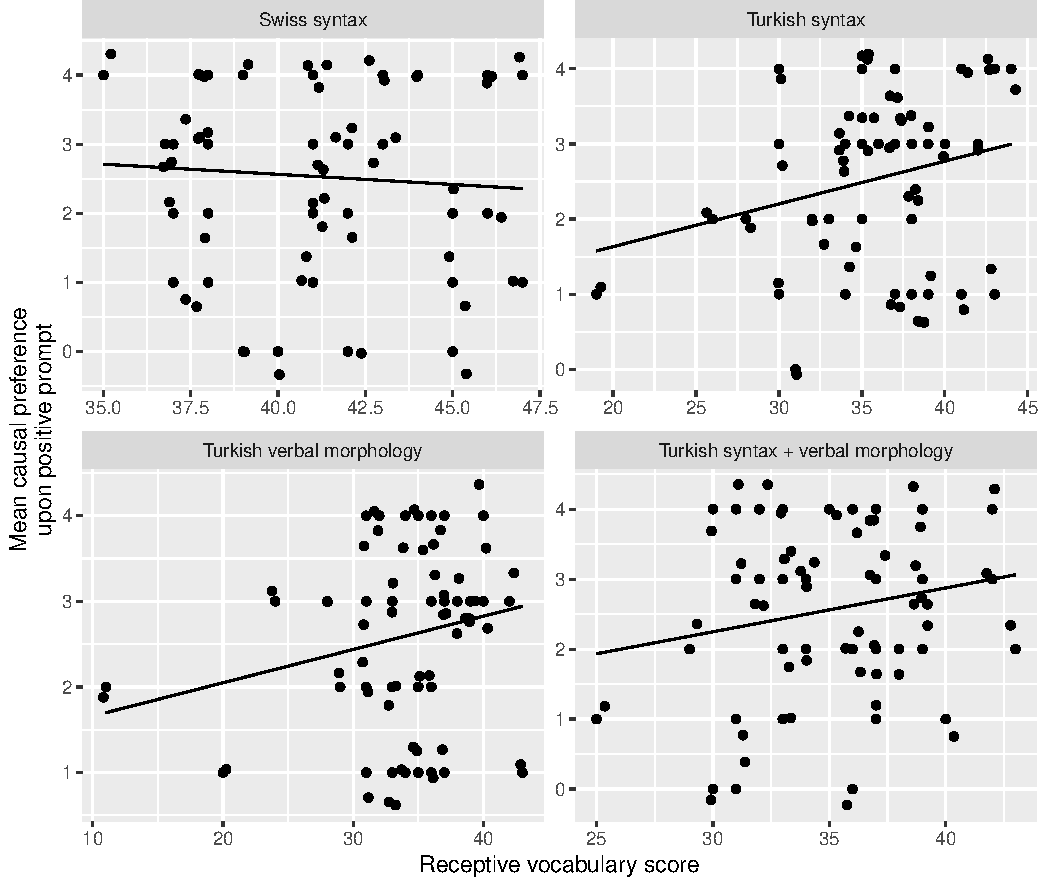
\includegraphics{fig1-1.pdf}
\caption{\label{fig:fig1}Scatterplot showing the
relationship between the causal preference upon the positive prompt and
receptive vocabulary scores across groups.}
\end{figure}

Next, we compared children's causal preference upon the positive prompt
in each group against chance (µ = 2). All groups chose the causal scene
upon the positive prompt at a level above chance (\emph{p}s = 0.012,
0.004, 0.001, 0.004; respectively for Swiss syntax, Turkish syntax,
Turkish verbal morphology, and Turkish syntax + verbal morphology
groups). To control that the children did not have a global causal
preference but that they selectively chose it upon the positive prompt,
we also compared children's causal preference upon the negative prompt
in each group against chance (µ = 2). All groups chose the causal video
upon the negative prompt at a level below chance (\emph{p}s = 0.000,
0.001, 0.000, 0.005; respectively for Swiss syntax, Turkish syntax,
Turkish verbal morphology, and Turkish syntax + verbal morphology
groups), showing that children were selectively mapping the causal
sentences onto causal events. Figure 2 plots the mean causal preference
of each group upon the positive and negative prompts. Together, these
results indicated that children in all language and cue groups made use
of the respective causality cues they were provided with to map onto
causal events, with no differences across the groups regarding the
extent to which they did so.

\begin{figure}[htbp]
\centering
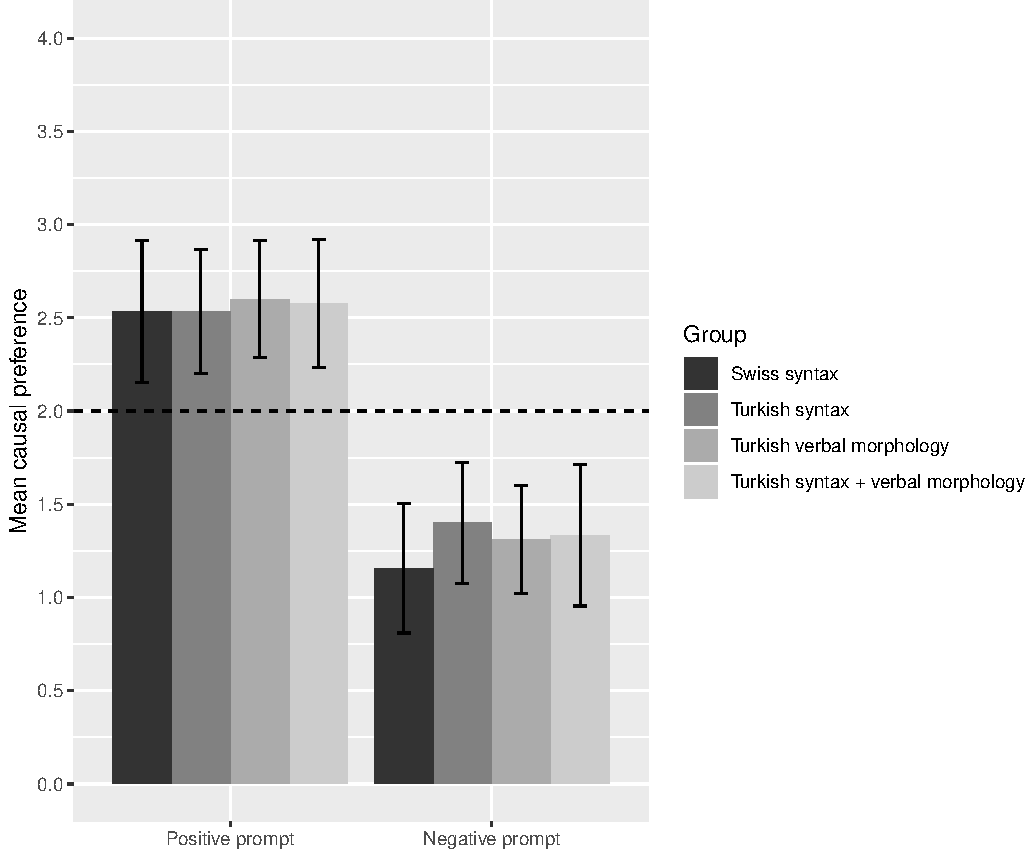
\includegraphics{fig2-1.pdf}
\caption{\label{fig:fig2}Children's causal preference upon
the positive and negative prompts across groups. Error bars represent
95\% confidence intervals.}
\end{figure}

In an exploratory vein, we also examined whether children who understood
the contact and the causality in the pretest videos performed better in
mapping the causal prompts onto causal scenes at test. Indeed, we found
that passing the pretest predicted children's causal preference upon the
positive prompt, controlling for the condition, age and the receptive
vocabulary score (\emph{t} = 2.40, \emph{p} = 0.02, Adjusted
R\textsuperscript{2} = 0.04), such that children who passed the pretest
were better in mapping causal prompts to causal scenes. In addition, the
causal preference score upon the positive prompt of those children who
failed the pretest were at chance for all groups (\emph{p}s = 0.15,1,
0.78, 0.19; respectively for Swiss syntax, Turkish syntax, Turkish
verbal morphology, and Turkish syntax + verbal morphology groups).
Figure 3 plots the mean causal preference upon the positive prompt for
children that passed or failed the pretest, across the groups.

\begin{figure}[htbp]
\centering
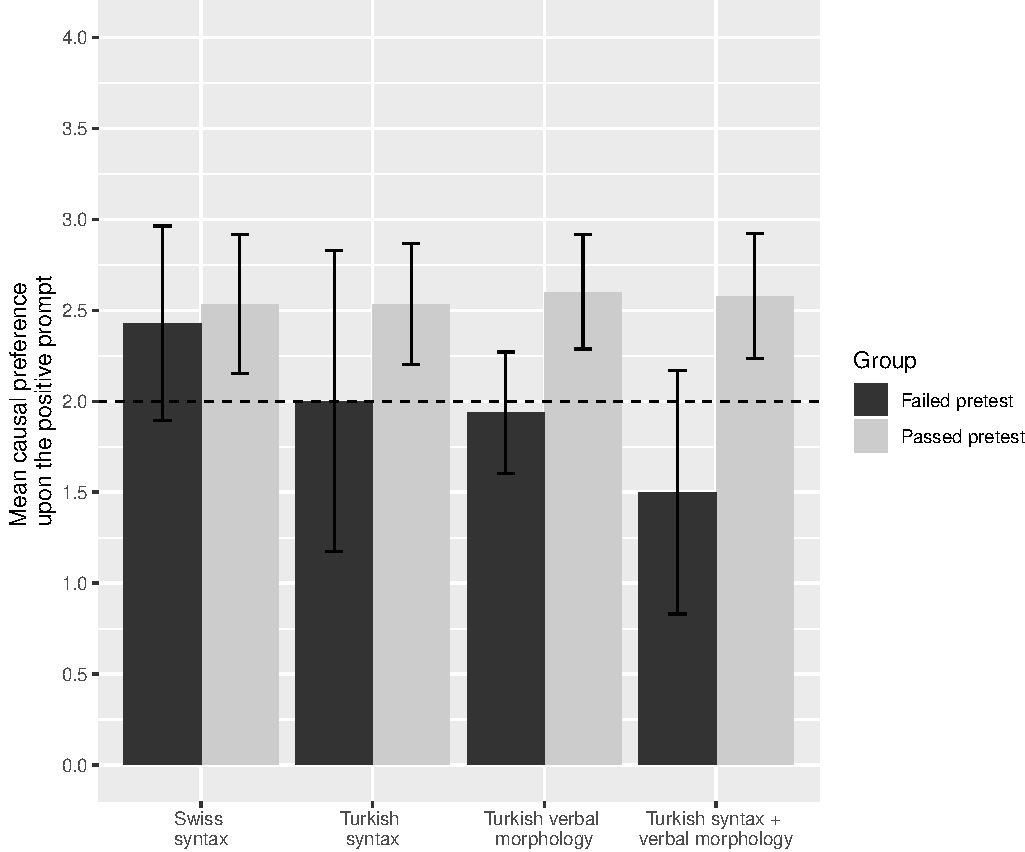
\includegraphics{fig3-1.pdf}
\caption{\label{fig:fig3}The causal preference upon the
positive prompt of children who passed or failed the pretest across
groups. Error bars represent 95\% confidence intervals.}
\end{figure}

\section{Discussion}\label{discussion}

In this study we assessed the influence of the syntactic frame and
verbal morphological cues to causality on deriving causal meanings in
two distinct languages with differing cue characteristics. We found that
the syntactic frame in Swiss-German were as good of a causality cue for
preschool children as the syntactic frame, the verbal morphology
(i.e.~causative marker) and the combination of the syntactic frame and
verbal morphology in Turkish. Hence, our findings suggest that the
syntactic frame is a strong, universal cue children benefit from to
derive causal meanings, evinced by the fact that even in Turkish, as a
language with pervasive noun ellipsis, children made use of it to a
similar extent as in Swiss-German, a language with intact two-argument
structure of causal sentences. Moreover, the language-specific verbal
causative marker in Turkish provided an exclusive but not supplementary
benefit. That is, without the syntax cue, Turkish children were still
able to map the sentence prompts with the causative marker to causal
scenes to a similar extent as Swiss children while they did not perform
any better when the causative marker was provided alongside the syntax
cue. Therefore, the verbal morphological cue might have compensated for
the lack of the syntactic cue. Overall, our findings suggest both
syntactic bootstrapping by Swiss-German as well as Turkish children and
morphological bootstrapping by Turkish children.

Syntactic frame as a causality cue is not always available in Turkish
due to noun ellipsis whereas it is always available in Swiss-German.
Nevertheless, Turkish children were able to make use of the transitive
syntax to infer causal meanings as accurately as the Swiss children, in
line with the previous studies showing the robustness of syntax as a
causality cue in languages that allow noun ellipsis (Göksun et al.,
2008; Lee \& Naigles, 2008). Could this tell us that the inherent
coupling between the transitive syntax and causal meaning is so strong
that the partial unavailability of this cue in Turkish does not disrupt
its efficiency of use as a cue? It is of course possible that the fewer
instances of learning opportunities with two argument sentences
depicting causal events with two participants are enough to generate a
generalization of \enquote{transitive frame equals causal meaning},
because this one-on-one mapping between the arguments of a sentence and
the participants of an event might be highly intuitive, robust and
resistant to occasional violations even in cases of noun ellipsis. On
the other hand, when the nouns are elided in causal sentences, it does
not mean that they go completely astray, leaving the child with no
information whatsoever to conjecture about the possible nouns of the
sentence. In most of the cases, the dropped arguments could be recovered
or inferred from the non-linguistic context, such as the object standing
in front of the listener or the discourse context, such as the noun
mentioned in the previous sentence. Therefore, the child might be
realizing the syntactic bootstrapping mechanism through learning to
reconstruct the complete argument structure by gathering all the
information surrounding the causal verb at hand (Küntay \& Slobin,
1996). In our experiment, the Turkish children in the condition with
only the verbal morphological cue might be complementing the sentence
\enquote{Kız nerde fezdirdi? (Where did the girl VERB-caus?)} in their
minds by means of the non-linguistic context, namely with the object
they see in the video (e.g.~the light box) such as \enquote{Kız nerde
\emph{feneri} fezdirdi? (Where did the girl VERB-caus \emph{the light
box}?)}

The causative marker in Turkish did not improve the mapping performance
of Turkish children when it was provided alongside the syntactic cue, in
comparison to Swiss children. However, when the causative marker was
provided in the absence of the syntactic cue, Turkish children still
performed as well as the Swiss children. If Turkish children relied
solely on the syntactic frame, then they would have chosen the causal
video at or below chance upon the prompt with the single noun phrase and
the causative marker (i.e. \enquote{The girl VERB-CAUS-PST}), given that
the intransitive frame cues a non-causal meaning (e.g. Naigles,
1990). Hence, children would have inferred that the girl does something
on her own and chosen one of the videos at chance since the girl
performs the same action such as hopping toward the toy in both the
causal and non-causal version of an event, or they would have further
inferred that the girl does something on her own but likely not on
another thing and chosen the causal video below chance. Therefore, the
verbal morphological cue in this condition is highly likely to have
driven the causal choices of the children. Yet, we acknowledge that the
effect of verbal morphology could be inferred more confidently by a
future study examining whether Turkish children would choose causal
scenes at or below chance when hearing a prompt with an intransitive
frame but without a causative marker.

Our findings do not fully support either of the proposed verb
acquisition theory's predictions in our comparisons. We cannot suggest a
universal precedence of the syntax cue on causal form to meaning mapping
since Turkish children were as good in the mapping of causal sentences
with only the verbal morphological cue as the Swiss children. We cannot
support an emergenist account either, while despite the lower validity
of the syntactic or verbal morphological cues per se in Turkish, Turkish
children did not perform differently than their Swiss counterparts who
entertained a higher validity of the syntactic cue. Thus, the input
characteristics did not play a major role in how strong a cue was
utilizded in mapping form to meaning. Nonetheless, a universalist
approach might be more likely to explain our findings, given that its
prediction only in our third question, that is the comparison between
Turkish verbal morphological group and the Swiss group, was not
confirmed. Based on this approach, we were expecting the Turkish
children to perform worse than Swiss children since the former were
lacking the syntactic cue. However, as discussed before, by the age of
three Turkish children might have learned to deal with the noun ellipsis
by recovering the missing nouns from the surrounding context.
Consequently, since all our event pairs involved the puppet and a toy,
the children might have complemented the sentences employing only the
subject (i.e. \enquote{the girl}) with the objects in the videos (e.g.
\enquote{the toy}) in their minds and still realized the syntactic cue.
However, we acknowledge that our predictions based on the universalist
and the emergenist accounts must be taken with caution, given that our
estimations of the availability of the morphological cues and the
prevalence of noun ellipsis in Turkish are only crude approximations.

With respect to the developmental trajectory of the causal form to
meaning mapping, we did not find an effect of age, in line with Kline et
al. (2017) who did not find a difference between 3- and 4-year-old
English-speaking children. The syntactic bootstrapping effect has
already been demonstrated with toddlers as young as 25 months of age (Naigles, 1990) and corroborated with an abundunce of studies scanning
toddler ages, although almost always with English speakers (see Fisher,
Gertner, Scott \& Yuan, 2010 for a review). Our findings show that by
the age of three, the syntactic bootstrapping effect is present in
speakers of Turkish and Swiss-German, as two understudied languages, as
well as the morphological bootstrapping effect in speakers of Turkish.
The causal and non-causal event alternatives in our task were attained
by manipulating the spatiotemporal contingencies between the two
sub-events of an action while keeping the sub-events the same in both causal
and non-causal versions. Hence, they were relatively more difficult to
distinguish than the obviously different event alternatives used in the
majority of the previous literature with younger children, that is,
caused motion events (causal) and simultaneous action events
(non-causal) (Fisher et al., 2010). Therefore, children in our study
were able to make use of any of the linguistic causality cues in their
respective languages to map onto rather complex causal scenes by the age
of three. It is an interesting fact that the performance did not improve
over the course of the 3rd and 4th year of life although it was not at
ceiling. The possibiliy remains that children still develop their
syntactic and verbal morphological analyses as well as their
understanding of causal and non-causal events further into the preschool
and school ages. In fact, especially for morphological analyses,
children do continue to develop their skills across the school ages for
morphologically rich (Durgunoğlu, 2003) as well as not so rich languages
(Berko, 1958).

The receptive vocabulary was related to the mapping performance only for
the Turkish children. One possibile explanation for the lack of this
relation in Swiss children is that their scores accumulated on the
higher end of the score range in our measurement scale so that we were
not able to capture the individual differences in their vocabulary
skills. It might be that the items of our vocabulary measurement tool
were more appropriate for the Swiss culture so that Swiss children
mostly scored high on this scale. Yet, the finding for the Turkish
children suggests that children with a larger vocabulary might entertain
more opportunities to deduce rules about the syntactic organization of
nouns and the operations with morphological markers simply because they
recognize these nouns in sentences and can determine their position in a
sentence as well as whehther they take any suffixes. However, our
vocabulary measure only consisted of nouns, hence we are limited in our
interpretations specifically for the verbal morphological markers. A
vocabulary measure of verbs would certainly serve as a better proxy for
the ability to distinguish root verbs and causative markers. Another
possibility is that the broader language skills of a child governs both
the lexicon and the syntactic and morphological analysis
skills\ldots{}\ldots{}

In an exploratory vein, we also compared the mapping performance of
children who passed the pretest and children who failed the pretest. We
found that the children who failed to learn the contact and causality
relations in the scenes of the pretest scored worse in mapping causal
sentences to causal scenes than those who did learn, and their
performance was only at chance level. This suggests that children can
make use of the linguistic cues of causality to match causal language
with causal events only when they can already distinguish causal and
non-causal events in their environment. It is possible that those
children who failed the pretest might have driven causal meanings from
the causal prompts and non-causal meanings from the non-causal prompts
but failed to match them correctly with the corresponding causal and
non-causal events because they were not able to detect the causality and
non-causality in the events although being trained. On the other hand,
it is also possible that the children who could understand the causality
cues in language were also already better in detecting the causality in
events.

\newpage

\section{References}\label{references}

\begingroup
\setlength{\parindent}{-0.5in} \setlength{\leftskip}{0.5in}

\hypertarget{refs}{}
\hypertarget{ref-R-citr}{}
Aust, F. (2018). \emph{Citr: 'RStudio' add-in to insert markdown
citations}. Retrieved from \url{https://CRAN.R-project.org/package=citr}

\hypertarget{ref-R-papaja}{}
Aust, F., \& Barth, M. (2018). \emph{papaja: Create APA manuscripts with
R Markdown}. Retrieved from \url{https://github.com/crsh/papaja}

\hypertarget{ref-bates1989functionalism}{}
Bates, E., MacWhinney, B., \& others. (1989). Functionalism and the
competition model. In \emph{The crosslinguistic study of sentence
processing} (Vol. 3, pp. 73--112).

\hypertarget{ref-berko1958child}{}
Berko, J. (1958). The child's learning of english morphology.
\emph{Word}, \emph{14}(2-3), 150--177.

\hypertarget{ref-bowerman2008crosslinguistic}{}
Bowerman, M., \& Brown, P. (2008). \emph{Crosslinguistic perspectives on
argument structure}. Taylor \& Francis.

\hypertarget{ref-chomsky1964aspects}{}
Chomsky, N. (1964). \emph{Aspects of the theory of syntax}.
MASSACHUSETTS INST OF TECH CAMBRIDGE RESEARCH LAB OF ELECTRONICS.

\hypertarget{ref-durgunouglu2003recognizing}{}
Durgunoğlu, A. Y. (2003). Recognizing morphologically complex words in
turkish. In \emph{Reading complex words} (pp. 81--92). Springer.

\hypertarget{ref-erguvanli1984function}{}
Erguvanli, E. E., \& Taylan, E. E. (1984). \emph{The function of word
order in turkish grammar} (Vol. 106). Univ of California Press.

\hypertarget{ref-fisher1996structural}{}
Fisher, C. (1996). Structural limits on verb mapping: The role of
analogy in children's interpretations of sentences. \emph{Cognitive
Psychology}, \emph{31}(1), 41--81.

\hypertarget{ref-fisher2002structural}{}
Fisher, C. (2002). Structural limits on verb mapping: The role of
abstract structure in 2.5-year-olds' interpretations of novel verbs.
\emph{Developmental Science}, \emph{5}(1), 55--64.

\hypertarget{ref-fisher1994better}{}
Fisher, C., Hall, D. G., Rakowitz, S., \& Gleitman, L. (1994). When it
is better to receive than to give: Syntactic and conceptual constraints
on vocabulary growth. \emph{Lingua}, \emph{92}, 333--375.

\hypertarget{ref-gampe2018bilex}{}
Gampe, A., Kurthen, I., \& Daum, M. M. (2018). BILEX: A new tool
measuring bilingual children's lexicons and translational equivalents.
\emph{First Language}, \emph{38}(3), 263--283.

\hypertarget{ref-gleitman1990structural}{}
Gleitman, L. (1990). The structural sources of verb meanings.
\emph{Language Acquisition}, \emph{1}(1), 3--55.

\hypertarget{ref-Goksun_etal2008a}{}
Göksun, T., Küntay, A. C., \& Naigles, L. R. (2008). Turkish children
use morphosyntactic bootstrapping in interpreting verb meaning.
\emph{Journal of Child Language}, \emph{35}(02), 291--323.

\hypertarget{ref-kabak2011turkish}{}
Kabak, B. (2011). Turkish vowel harmony. \emph{The Blackwell Companion
to Phonology}, 1--24.

\hypertarget{ref-ketrez2004children}{}
Ketrez, F. N. (2004). Children's accusative case and indefinite objects.
\emph{Dilbilim Arastirmalari}, \emph{2004}, 63--74.

\hypertarget{ref-kline2017linking}{}
Kline, M., Snedeker, J., \& Schulz, L. (2017). Linking language and
events: Spatiotemporal cues drive children's expectations about the
meanings of novel transitive verbs. \emph{Language Learning and
Development}, \emph{13}(1), 1--23.

\hypertarget{ref-kuntay1996listening}{}
Küntay, A., \& Slobin, D. I. (1996). Listening to a turkish mother: Some
puzzles for acquisition.

\hypertarget{ref-landau2009language}{}
Landau, B., Gleitman, L. R., \& Landau, B. (2009). \emph{Language and
experience: Evidence from the blind child} (Vol. 8). Harvard University
Press.

\hypertarget{ref-lee2005input}{}
Lee, J. N., \& Naigles, L. R. (2005). The input to verb learning in
mandarin chinese: A role for syntactic bootstrapping.
\emph{Developmental Psychology}, \emph{41}(3), 529.

\hypertarget{ref-lee2008mandarin}{}
Lee, J. N., \& Naigles, L. R. (2008). Mandarin learners use syntactic
bootstrapping in verb acquisition. \emph{Cognition}, \emph{106}(2),
1028--1037.

\hypertarget{ref-lidz2003understanding}{}
Lidz, J., Gleitman, H., \& Gleitman, L. (2003). Understanding how input
matters: Verb learning and the footprint of universal grammar.
\emph{Cognition}, \emph{87}(3), 151--178.

\hypertarget{ref-naigles1990children}{}
Naigles, L. (1990). Children use syntax to learn verb meanings.
\emph{Journal of Child Language}, \emph{17}(2), 357--374.

\hypertarget{ref-naigles1993first}{}
Naigles, L. G., \& Kako, E. T. (1993). First contact in verb
acquisition: Defining a role for syntax. \emph{Child Development},
\emph{64}(6), 1665--1687.

\hypertarget{ref-naigles2002language}{}
Naigles, L. R., \& Lehrer, N. (2002). Language-general and
language-specific influences on children's acquisition of argument
structure: A comparison of french and english. \emph{Journal of Child
Language}, \emph{29}(3), 545--566.

\hypertarget{ref-naigles2006language}{}
Naigles, L. R., Küntay, A. C., Göksun, T., \& others. (2006).
Language-specific properties influence childrens acquisition of argument
structure.

\hypertarget{ref-peirce2018building}{}
Peirce, J., \& MacAskill, M. (2018). \emph{Building experiments in
psychopy}. Sage.

\hypertarget{ref-pinker2009language}{}
Pinker, S. (2009). \emph{Language learnability and language development,
with new commentary by the author} (Vol. 7). Harvard University Press.

\hypertarget{ref-R-base}{}
R Core Team. (2019). \emph{R: A language and environment for statistical
computing}. Vienna, Austria: R Foundation for Statistical Computing.
Retrieved from \url{https://www.R-project.org/}

\hypertarget{ref-rispoli1995missing}{}
Rispoli, M. (1995). Missing arguments and the acquisition of predicate
meanings. \emph{Beyond Names for Things: Young Children's Acquisition of
Verbs}, 331--352.

\hypertarget{ref-R-broom}{}
Robinson, D., \& Hayes, A. (2019). \emph{Broom: Convert statistical
analysis objects into tidy tibbles}. Retrieved from
\url{https://CRAN.R-project.org/package=broom}

\hypertarget{ref-shibatani2002causative}{}
Shibatani, M., \& Pardeshi, P. (2002). The causative continuum.
\emph{Typological Studies in Language}, \emph{48}, 85--126.

\hypertarget{ref-ural2009morphological}{}
Ural, A. E., Yuret, D., Ketrez, F. N., Koçbaş, D., \& Küntay, A. C.
(2009). Morphological cues vs. number of nominals in learning verb types
in turkish: The syntactic bootstrapping mechanism revisited.
\emph{Language and Cognitive Processes}, \emph{24}(10), 1393--1405.

\hypertarget{ref-R-ggplot2}{}
Wickham, H. (2016). \emph{Ggplot2: Elegant graphics for data analysis}.
Springer-Verlag New York. Retrieved from
\url{https://ggplot2.tidyverse.org}

\hypertarget{ref-R-usethis}{}
Wickham, H., \& Bryan, J. (2019). \emph{Usethis: Automate package and
project setup}. Retrieved from
\url{https://CRAN.R-project.org/package=usethis}

\hypertarget{ref-R-dplyr}{}
Wickham, H., François, R., Henry, L., \& Müller, K. (2019). \emph{Dplyr:
A grammar of data manipulation}. Retrieved from
\url{https://CRAN.R-project.org/package=dplyr}

\hypertarget{ref-R-devtools}{}
Wickham, H., Hester, J., \& Chang, W. (2019). \emph{Devtools: Tools to
make developing r packages easier}. Retrieved from
\url{https://CRAN.R-project.org/package=devtools}

\hypertarget{ref-R-knitr}{}
Xie, Y. (2015). \emph{Dynamic documents with R and knitr} (2nd ed.).
Boca Raton, Florida: Chapman; Hall/CRC. Retrieved from
\url{https://yihui.name/knitr/}

\bibliographystyle{apacite}
\bibliography{causality.bib}
\endgroup

\end{document}
